\usetikzlibrary{arrows}
\usetikzlibrary{calc}

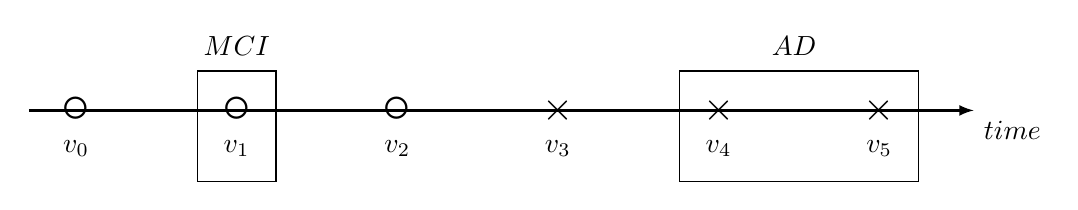
\begin{tikzpicture}[scale=1, line/.style={>=latex}] 

	\coordinate (t0) at (0, 0);
	\coordinate (t1) at (12, 0);
	\coordinate (dummy) at (0, 4);

	\draw[->, line, color=black, thick]
		(t0) --
			node [pos=0.05, below=-8.5pt] {\huge $\circ$}
			node [pos=0.05, below=7pt] {$v_0$}
			node [pos=0.22, below=-8.5pt] {\huge $\circ$}
			node [pos=0.22, below=7pt] {$v_1$}
			node [pos=0.22, above=16pt] {$MCI$}
			node [pos=0.39, below=-8.5pt] {\huge $\circ$}
			node [pos=0.39, below=7pt] {$v_2$}
			node [pos=0.56] {\Large $\times$}
			node [pos=0.56, below=7pt] {$v_3$}
			node [pos=0.73] {\Large $\times$}
			node [pos=0.73, below=7pt] {$v_4$}
			node [pos=0.81, above=16pt] {$AD$}
			node [pos=0.90] {\Large $\times$}
			node [pos=0.90, below=7pt] {$v_5$}
			node [at end, below right] {$time$}
		(t1);

	\draw[draw=black] (2.14,0.5) rectangle ++ (1,-1.4);
	\draw[draw=black] (8.26,0.5) rectangle ++ (3.04,-1.4);
	
	%\draw[->, line, color=black, very thick] (t0) -- node [at end] {$\circ$} (dummy);

\end{tikzpicture}


